\documentclass{frontiersSCNS}
\usepackage{url,hyperref,lineno,microtype,subcaption}
\usepackage[onehalfspacing]{setspace}
\usepackage{float}


\linenumbers

\usepackage[utf8]{inputenc}
\floatplacement{figure}{H}

\def\keyFont{\fontsize{8}{11}\helveticabold }
\def\firstAuthorLast{Villaseñor-Derbez {et~al.}}
\def\Authors{Juan Carlos Villaseñor-Derbez\(^{1,*}\), Eréndira
Aceves-Bueno\(^{1,*}\), Álvin Suarez-Castillo\(^{2}\), Stuart
Fulton\(^{2}\), Jorge Torre\(^{2}\)}
% Affiliations should be keyed to the author's name with superscript numbers and be listed as follows: Laboratory, Institute, Department, Organization, City, State abbreviation (USA, Canada, Australia), and Country (without detailed address information such as city zip codes or street names).
% If one of the authors has a change of address, list the new address below the correspondence details using a superscript symbol and use the same symbol to indicate the author in the author list.
\def\Address{\(^{1}\)Bren School of Environmental Science and Management, University
of California, Santa Barbara, Santa Barbara, CA,
USA\newline \(^{2}\)Comunidad y Biodiversidad A.C., Guaymas, Mexico}
% The Corresponding Author should be marked with an asterisk
% Provide the exact contact address (this time including street name and city zip code) and email of the corresponding author
\def\corrAuthor{Juan Carlos Villaseñor-Derbez, Bren Hall, University of California,
Santa Barbara, Santa Barbara, CA, 93106}

\def\corrEmail{\href{mailto:jvillasenor@bren.ucsb.edu}{\nolinkurl{jvillasenor@bren.ucsb.edu}}}

\usepackage{amsthm}
\newtheorem{theorem}{Theorem}[section]
\newtheorem{lemma}{Lemma}[section]
\theoremstyle{definition}
\newtheorem{definition}{Definition}[section]
\newtheorem{corollary}{Corollary}[section]
\newtheorem{proposition}{Proposition}[section]
\theoremstyle{definition}
\newtheorem{example}{Example}[section]
\theoremstyle{definition}
\newtheorem{exercise}{Exercise}[section]
\theoremstyle{remark}
\newtheorem*{remark}{Remark}
\newtheorem*{solution}{Solution}
\begin{document}
\onecolumn
\firstpage{1}

\title[Community-based marine reserves]{Management and effectiveness of community-based marine reserves in
small-scale fisheries} 

\author[\firstAuthorLast ]{\Authors} %This field will be automatically populated
\address{} %This field will be automatically populated
\correspondance{} %This field will be automatically populated

\extraAuth{}

\maketitle



\begin{abstract}

Al finalizar revisiones




\medskip
\tiny
 \keyFont{ \section{Keywords:} Marine Protected Areas, Marine Conservation, Small-Scale Fisheries,
Citizen Science, Mexico, Social-Ecological Systems}



\end{abstract}


\textbf{Last update}: 2018-06-08

\clearpage

\section{Introduction}\label{introduction}

Marine ecosystems around the world sustain significant impacts due to
overfishing and unsustainable fishing practices
\citep{halpern_2008-dK,worm_2006-IB,pauly_2005-qV}. A common approach to
manage the spatial distribution of fishing effort to recover stocks and
preserve biodiversity is through the implementation of marine reserves
(MRs). These areas allow bounded populations to recover by limiting all
extractive activities \citep{halpern_2002}. The science of MRs has
largely focused on understanding the ecological effects of these areas,
which include increased biomass, richness, and densities of organisms
within the protected regions, climate change mitigation, and protection
from environmental variability
\citep{lester_2009-Ks,giakoumi_2017-V2,sala_2017-69,roberts_2017-J9,micheli_2012-EU}.
Modelling studies show that the fishery benefits of marine reserves
depend on initial stock status and the type of management under which
the fishery operates \citep{hilborn_2006}, as well as reserve size and
the amount of larvae exported from these \citep{krueck_2017-J1}. Other
research has focused on the relationship between socioeconomic and
governance structures and their relationship to ecological effectiveness
\citep{halpern_2013,lpezangarita_2014,mascia_2017-m_}. However, few
studies simultaneously evaluate MRs from all these perspectives
(\emph{e.g.} \citet{lpezangarita_2014}).

While ecological factors like habitat representation within the MR or
connectivity to other areas can determine the success of a MR, its
effectiveness also depends on the socioeconomic and governance settings
under which they are implemented and managed. Literature shows that many
non-ecological characteristics can play an equally important role in the
effectiveness of MRs. For example, age of a reserve (\emph{i.e.} time
since its implementation) and size were key to the effectiveness of MRs
in Palau \citep{friedlander_2017-oI}. In the Mediterranean,
\citet{difranco_2016-Xw} identify that surveillance and enforcement,
presence of a management plan, and involvement of fishers in management
and decision--making along with promotion of sustainable fishing
practices were the key factors that increased stock health and income to
fishers. At a global level, enforcement, age, size, and isolation are
important factors that determine the effectiveness of the reserves
\citep{edgar_2014-UO}. However, MRs represent part of a more complex
social-ecological systems governed by the interaction between humans and
the environment. In this work we evaluate community-based marine
reserves in Mexico using a triple bottom line approach by using
ecological, socioeconomic, and governance indicators that provide a
holistic view of the reserves \citep{halpern_2013}.

There are three main approaches to implement MRs, each of which have its
pros and cons. We describe them in the context of Mexican MRs, but argue
that at least the first two apply elsewhere. MRs were historically
implemented and managed by a government agency, in this case the
National Commission of Protected Areas (\emph{Comisión Nacional de Áreas
Marinas Protegidas}, CONANP). While CONANP has made efforts to have a
participatory process, the implementation of these zones is still mainly
a top-down process. A second approach is the implementation of
community-based marine reserves within areas of exclusive access
(\emph{i.e.} TURFs), thus making them TURF-reserves
\citep{afflerbach_2014-HP}. Community-based spatial closures ocurr in
other places, like the \emph{kapu} or \emph{ra'ui} areas in the Pacific
Islands \citep{bohnsack_2004,johannes_2002}. This bottom-up approach
increases compliance and self-enforcement
\citep{gelcich_2015-Gw,espinosaromero_2014-PY,beger_2004-Y8}. However,
these lack legal recognition and rely on the exclusive access granted by
the TURF, making it impossible to enforce without one. In an effort to
provide a legal framework for these reserves, Civil Society
Organizations (CSOs) served as the bridge between fishers and
government. In 2014, a new norm \citep{nom} allowed fishers to request
the legal recognition of a community-based reserve under the name of
``Fishing Refugia'' (\emph{Zona de Refugio Pesquero}). These can be
implemented as temporal or partial eservs, which can protect one, some,
or all resources within them. Since then, \textbf{39} of these have been
implemented along the Pacific, Gulf of California, and Mexican Caribbean
coastlines, but no formal evaluation of their effectiveness has taken
place.

This work combines causal inference techniques and the social-ecological
systems framework to provide a holistic evaluation of community-based
marine reserves in three coastal communities in Mexico. The objective of
this work is twofold. First, provide a triple bottom line evaluation of
the effectiveness of community-based marine reserves that can inform
similar processes in other countries. And second, perform the first
formal evaluation of Fishing Refugia in Mexico and identify areas where
improvement or adjustment might result in increased effectiveness. On
both cases, we draw from the lessons learned and provide management
recommendations to ensure or improve the effectiveness of
community-based marine reserves.

\section{Materials and Methods}\label{materials-and-methods}

\subsection{Study area}\label{study-area}

We evaluate community-based marine reserves from three coastal
communities located in the Pacific coast of Baja California and the
Mexican Caribbean (Fig \ref{fig:map}). All communities are organized as
fishing cooperatives that hold Territorial Use Rights for Fisheries
(TURFs). Isla Natividad (IN) lies west of the Baja California Peninsula
(Fig \ref{fig:map}B), where kelp forests and rocky reefs are the
predominant habitats. The island is home to the \emph{Sociedad
Cooperativa de Producción Pesquera (SCPP) Buzos y Pescadores de la Baja
California}, whose main resource by value is the spiny lobster
(\emph{Panulirus interruptus}). However, other resources like finfish
(yellow-tail jack, \emph{Seriola lalandi}), sea cucumber
(\emph{Parastichopus parvimensis}), red sea urchin (\emph{Mesocentrotus
franciscanus}), snail (\emph{Megastraea turbanica} y \emph{M. undosa}),
and abalone (\emph{Haliotis spp}) are also important sources of income.
In 2006, the community decided to implement two community-based marine
reserves within their fishing grounds to protect commercially important
invertebrate species (mainly lobster and abalone). Until today, these
reserves are yet to be legally recognized as Fishing Refugia but count
with full support from the community.

The other two communities are Maria Elena (ME) and Punta Herrero (PH;
Fig \ref{fig:map}C) in the Yucatan Peninsula, where coral reefs and
mangroves are the representative coastal ecosystems. ME is a fishing
camp --visited intermitently during the fishing season-- belonging to
the Cozumel fishing cooperative (\emph{SCPP Cozumel}); PH is home to the
\emph{SCPP José María Azcorra} cooperative. Their main fishery is the
Caribbean spiny lobster (\emph{Panulirus argus}), but they also target
finfish in the off season, mainly snappers (Lutjanidae) and groupers
(Serranidae). ME established eight marine reserves in 2012, and PH
established four marine reserves in 2013 and an additional
community-based (\emph{i.e.} not legally recognized). All these reserves
are legally recognized as Fishing Refugia.

\subsection{Data collection}\label{data-collection}

We use three main sources of information to evaluate these reserves.
Ecological data come from the annual ecological monitoring of reserve
and control areas, carried out by members from each community and
personnel from the Mexican CSO \emph{Comunidad y Biodiversidad}
(\href{www.cobi.org.mx}{COBI}). Trained divers record richness and
abundances of fish and invertebrate species in the reserves and control
sites. Size structures are also collected for fish evaluations. We
define control sites as regions with habitat characteristics similar to
the corresponding reserves, and that presumably had a similar
probability of being selected as reserves during the design phase. We
focus our evaluation for sites where data are avaialable for reserve and
control sites, before and after the implementation of the reserve. This
provides us with a Before-After-Control-Impact (\emph{i.e.} BACI)
sampling design that allows us to capture and control for temporal and
spatial dynamics \citep{depalma_2018,ferraro_2006-oW}. BACI designs and
causal inference techniques have proven effective to evaluate marine
reserves, as they allow us to causally attribute observed changes to the
intervention \citep{moland_2013-VP,Villasenor-Derbez_2018}. All sites
were surveyed annually, and at least once before implementation of the
reserves. Table \ref{table:com_sum} shows a summary of the reserves
included in this study.

\begin{figure}
\centering
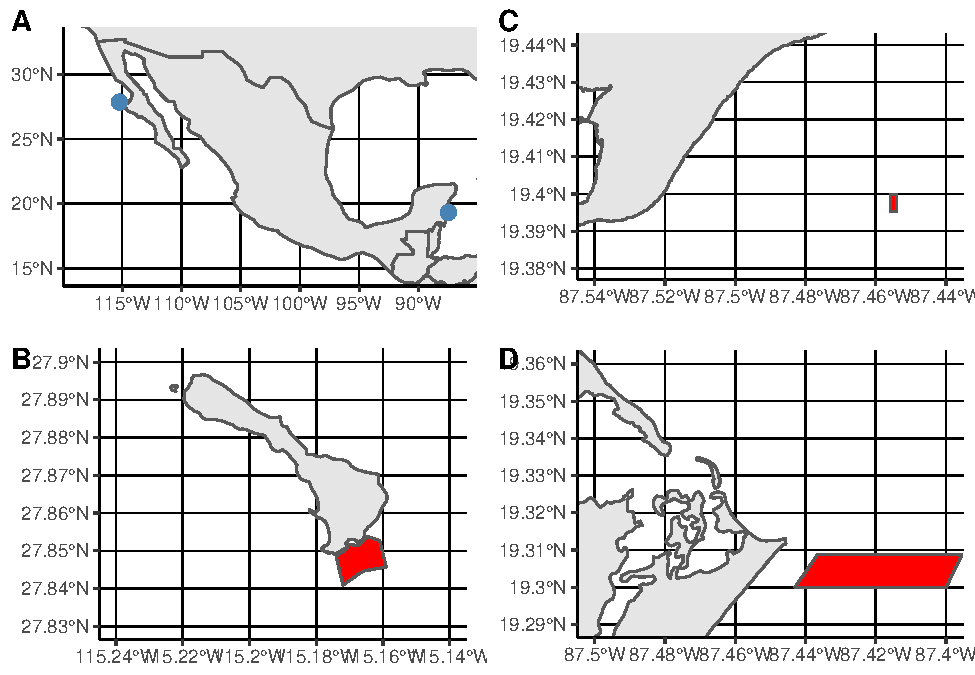
\includegraphics{Villasenor-Derbez_files/figure-latex/unnamed-chunk-1-1.pdf}
\caption{\label{fig:unnamed-chunk-1}\label{fig:map}Location of the three
coastal communities studied (A). Isla Natividad (B) is located off the
Baja California Peninsula, Maria Elena (C) and Punta Herrero (D) are
located in the Yucatan Peninsula. Blue polygons represent the TURFs, and
red polygons the marine reserves.}
\end{figure}

\begin{table}

\caption{\label{tab:unnamed-chunk-2}\label{table:com_sum} Summary of commuity--based marine reserves by community.}
\centering
\begin{tabular}[t]{l|r|r|r|r}
\hline
Community & TURF area ($km^2$) & Reserve area ($km^2$) & Percent as reserves & Year of implementation\\
\hline
Isla Natividad & 889.5 & 1.53 & 0.1720067 & 2006\\
\hline
Maria Elena & 353.1 & 0.10 & 0.0283206 & 2012\\
\hline
Punta Herrero & 299.7 & 0.43 & 0.1434768 & 2013\\
\hline
\end{tabular}
\end{table}

Socioeconomic data come from landing receipts reported to the National
Commission for Aquaculture and Fisheries (\emph{Comisión Nacional de
Acuacultura y Pesca}; CONAPESCA). Data contain monthly lobster landings
(Kg) and value (MXP) from 2000 to 2014 for cooperatives with and without
marine reserves (\textbf{Fig S1}). This information was aggregated by
year, and economic values were adjusted by the Consumer Price Index
\citep{oecd_2017-VV} as:

\begin{equation}
I_t = RI_t\times\frac{CPI_t}{CPI_T}
\label{eqn:cpi}
\end{equation}

Where \(I_t\) represents the adjusted income for year \(t\) as the
product between the reported income for that year and the ratio between
the consumer price index in that year (\(CPI_t\)) to the most recent
year's consumer price index (\(CPI_T\)).

Data for the qualitative analysis of the social-ecological system were
collected at the community--level from official documents used in the
creation and designation of the marine reserves
\citep{dof_website_2012,dof_website_2013} and based on the authors'
experience and knowledge of the communities. These include information
on the resource system, the resource units, actors, and the governance
system itself (\textbf{S1 Table}).

\subsection{Data analysis}\label{data-analysis}

We evaluate the effect that marine reserves have had on four biological
and two socioeconomic indicators (Table \ref{table:indicators}). Recall
that reserves were implemented to protect lobster and other benthic
invertebrates. However, we also use the available fish data, since
finfish are targeted in the off-season and because there might be
associated cobenefits of the reserve.

\begin{table}[H]

\caption{\label{tab:unnamed-chunk-3}\label{table:indicators}List of indicators used to evaluate the effectiveness of marine reserves, grouped by category.}
\centering
\begin{tabular}[t]{l|l|l}
\hline
Category & Indicador & Units\\
\hline
Biological & Lobster density & org / $m^2$\\
\hline
Biological & Invertebrate density & org / $m^2$\\
\hline
Biological & Fish biomass & Kg / $m^2$\\
\hline
Biological & Fish density & org / $m^2$\\
\hline
Socioeconomic & Income from target species & M MXP\\
\hline
Socioeconomic & Landings from target species & Metric Tonnes\\
\hline
\end{tabular}
\end{table}

We use a difference-in-differences analysis to evaluate the biological
indicators. This approach allows us to estimate the effect that the
reserve has on the biological indicators by comparing trends across time
and treatments (\emph{i.e.} reserve / control sites
\citet{moland_2013-VP,Villasenor-Derbez_2018}). The analysis is
performed with a multiple linear regression of the form:

\begin{equation}
I_{itj} = \alpha + \gamma_{t} Year_t + \beta Zone_i + \lambda_{t} Year_t\times Zone_i + \sigma_jSpp_j + \epsilon
\label{eqn:reg_bio}
\end{equation}

Where year-fixed effects are represented by \(\gamma_{it} Year_t\), and
\(\beta Zone_i\) captures the difference between reserve (\(Zone = 1\))
and control (\(Zone = 0\)) sites. The interaction term
\(\lambda_{it} Year_t\times Zone_i\) represents the mean change in the
indicator inside the reserve, for year \(t\), with respect to the year
of implementation in the control site (See Table \ref{table:com_sum}).
When evaluating biomass and densities of the entire benthic or fsh
communities, we include \(\sigma_j\) to control for species-fixed
effects.

Socioeconomic indicators are evaluated with a similar approach (Eq
\ref{eqn:soc_reg}). Due to data constrains, only Isla Natividad and
Maria Elena are evaluated in this case. We constructed panel-data
information with yearly (2001 - 2014) lobster landings and income of the
studied and neighbouring communities that have similar management
strategies, and belong to larger Cooperative Federtations
\citep{mccay_2017-1m,ayer_2018}. Neighbouring communities are used as
counterfacutals that allow us to control for unobserved time-invariants.
Each ``treated'' community (Isla Natividad and Maria Elena) has three
counterfactual communities.

\begin{equation}
I = \alpha + \gamma_{t} Year_t + \beta Treated_i + \lambda_{t} Year_t\times Treated_i + \sigma_jCom_j +\epsilon
\label{eqn:soc_reg}
\end{equation}

The model interpretation remains as for Eq \ref{eqn:reg_bio}, but in
this case the \(Treated\) dummy variable indicates if the community has
a reserve (\(Treated = 1\)) or not (\(Treated = 0\)) and \(\sigma_jCom\)
captures community-level fixed-effects. These regressions allows us to
make a causal link between the implementation of marine reserves and the
observed trends by accounting for temporal and spatial dynamics
\citep{depalma_2018}. The effect of the reserve is captured by the
\(\lambda_t\) coefficient, and represents the difference observed
between the control site before the implementation of the reserve and
the treated sites at time \(t\) after controlling for other time and
space variations (\emph{i.e.} \(\gamma_t\) and \(\beta\) respectively).
All model coefficients were estimated via ordinary least-squares and
heteroskedastic-robust standard errors \citep{zeileis_2004-7n}. All
analyses were performed in R 3.5.0 and R Studio 1.1.453 \citep(R\_2018).

\section{Results}\label{results}

The following sections present the effect that marine reserves had on
each of the biological and socioeconomic indicators for each coastal
community. Results are presented in terms of the difference through time
and across sites, relative to the control site on the year of
implementation (\emph{i.e.} effect size \(\lambda_t\)). We also provide
an overview of the governance settings of each community, and discuss
how these dimensions might be related to the effectiveness of the
reserves.

\subsection{Biological}\label{biological}

Indicators showed idiosyncratic responses through time for each
community. Figure \ref{fig:indicators}A shows positive effect sizes for
lobster densities for Isla Natividad and Punta Herrero during the first
years, but the effect is eroded through time. These effects are in the
order of 0.2 extra organisms \(m^{-2}\) but are not significantly
different from zero (\(p > 0.05\)). Lobster densities were only
significantly positive for Isla Natividad on the sixth year (\emph{i.e.}
2012; \(p < 0.05\)), a year after the hypoxia events described by
\citet{micheli_2012-EU} caused mass mortality of organisms. Likewise, no
changes were detected in fish biomass or invertebrate and fish densities
(\ref{fig:indicators}B-D), where effect sizes oscillated around zero
without clear trends. Full tables with model coefficients are presented
in the supplementary materials (\textbf{S2 Table}, \textbf{S3 Table},
\textbf{S4 Table}).

\subsection{Socioeconomic}\label{socioeconomic}

Lobster landings and revenue were only available for Isla Natividad and
Maria Elena (Fig \ref{fig:lobsters}). For all years befor
implementation, the effect sizes are close to zero, indicating that the
control and treatment sites track each other well and that these are
plausible controls. However, effect sizes do not change after the
implementation of the reserve. Again, the negative coeficient observed
for Isla Natividad on year 5 correspond to the 2011 hypoxia events. The
only positive change observed in lobster landings is for Isla Natividad
in 2014 (\(p < 0.1\)). The trhee years of post-implementation data for
Maria Elena do not show a significant effect of the reserve. Isla
Natividad shows higher revenues after the iumplementation of the
reserve, as compared to the control communities. However, these changes
are also not ignificantly different and present an increased variation.
All regression coefficients for each community and indicator are
presented in \textbf{S5 Table}.

\subsection{Governance}\label{governance}

Although we have little information on the social dimension of these
fisheries, we can use the social-ecologycal systems framework
(\textbf{S1 Table}) to analyze the performance of each governance system
(\textbf{S6 Table}).

Our analysis shows that all of the systems analyzed share similarities
in their Governance system which is based on cooperatives (GS5.2.3.2),
with strong rules in use that include Operational rules (GS6.2),
Collective-choice rules (GS6.3), Constitutional rules (GS6.3), and even
Territorial use communal rights (GS6.1.4.3). However, we identified
important differences in terms of the actors, resource systems and
resource units. The value of lobster in isla natividad is higher than
the lobster sold from Punta Herrero and Maria Elena (RU4), which can
reduce the pressure on harvest. Lastly, in terms of actors, although all
communities show a high level of leadership (A5), the level of trust
(A6.1) is lower in Punta Herrero. In general, the presence and success
of conservation initiatives depends on the incentives of local
communities to maintain a healthy status of the resources they depend
upon \citep{jupiter_2017}. The enabling conditions for conservation seem
to be strongly present in all communities. Due to the clarity of access
rights and isolation, the benefits of conservation directly benefit the
members of the fishing cooperative. These conditions have favored the
development of an efficient community-based enforcement systems.

\clearpage

\begin{figure}
\centering
\includegraphics{Villasenor-Derbez_files/figure-latex/unnamed-chunk-4-1.pdf}
\caption{\label{fig:unnamed-chunk-4}\label{fig:indicators}Effect sizes for
marine reserves from Isla Natividad (IN; red cirlcles), Maria Elena (ME;
blue triangles), and Punta Herrero (PH; green squares) for lobster
densities (\emph{Panulirus spp}; A), fish biomass (B), invertebrate
densities (C), and fish densities (D). Plots are ordered by survey type
(left column: invertebrates; right column: fish). Points are jittered
hotizontally to avoid overplotting. Points indicate the effect size, and
errorbars standard errors. Years have been centered to year of
implementation.}
\end{figure}

\begin{figure}
\centering
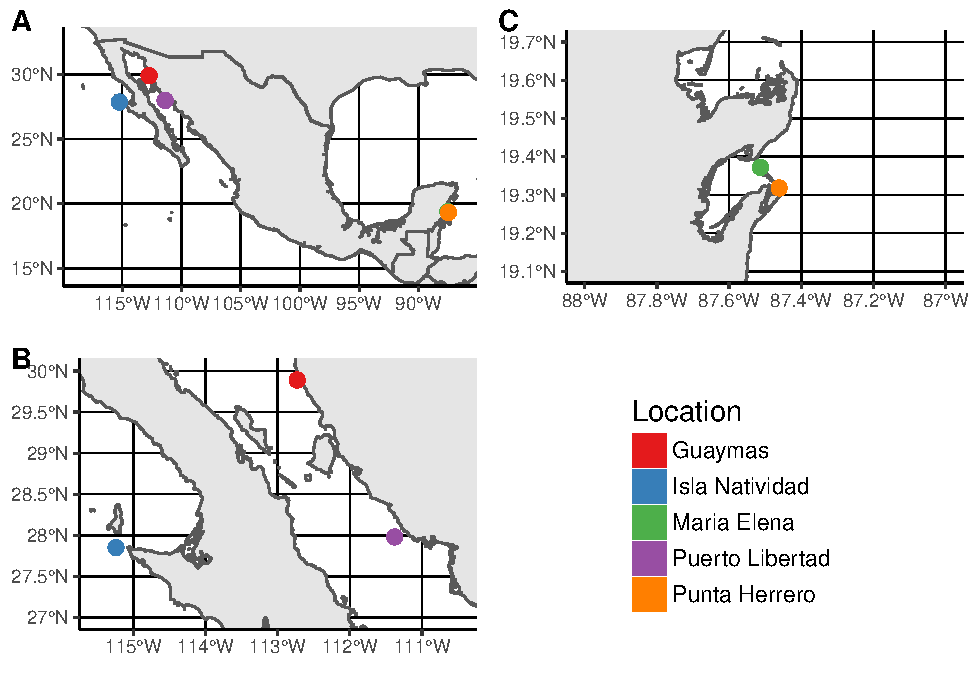
\includegraphics{Villasenor-Derbez_files/figure-latex/unnamed-chunk-6-1.pdf}
\caption{\label{fig:unnamed-chunk-6}\label{fig:lobsters}Effect sizes for
lobster catches (A) and revenues (B) in at Isla Natividad (IN; red
circles) and Maria Elena (ME; blue triangles)}
\end{figure}

\clearpage

\section{Discussion}\label{discussion}

Our results indicate that marine reserves are ineffective in increaseing
population sizes of lobsters in the three communities. The socioeconomic
indicators pertaining to landings and revenues showed little to no
change after reserve implementation. While lobster densities represent
an indicator directly tied to reserve objectives, we also evaluate other
biological indicators to test for additional effects and fail to detect
any effect other then the already reported buffering effect that
Natividad reserves can have to environmental variability
\citep{micheli_2012-EU}. The lack of expected effectiveness poses the
question, why do these communities continue to support the reserves?
Understanding the social-ecological context in which these communities
and their reserves operate might provide insights to this question.
Here, we discuss plausible explanations to lack of effectiveness
observed onthe biological and socioeconomic indicators based on our
social-ecological system analysis. We also discuss potential
shortcomings in our analysis, and provide management recommendations to
improve reserve effectiveness.

Our approach to evaluate the temporal and spatial changes of each
indicator provides a more robust measure of reserve effectiveness. Some
works have solely focused on an inside-outside comparison of indicators
\citep{guidetti_2014-8Z,friedlander_2017-oI,rodriguez_2017-PD}, which do
not address temporal variability \citep{depalma_2018}. Other works have
compared the trend observed within a reserve through time
\citep{betti_2017-lq}, which cannot distinguish between the temporal
trends in a reserve and the entire system \citep{depalma_2018}. By
accounting for trends between sites and through time, we can control for
time and space dynamics, and provide a better identification of the
effect.

Age, isolation, and enforcement are important factors influencing
effectiveness of a marine reserve \citep{edgar_2014-UO}. Isla Natividad
has the oldest reserve, is fairly isolated, and has a well-established
community-based enforcement system. Neighbouring fishing communities are
known to be well organized with successful resource management of their
resources \citep{mccay_2017-1m,mccay_2014-CN}. Maria Elena and Punta
Herrero are relatively young reserves (Table \ref{table:com_sum}). With
the age, relative isolation, and enforcement level of these reserves,
one would expect to observe effectiveness. However, another key feature
of effective MRs is size \citep{edgar_2014-UO}; the lack of
effectiveness is perhaps attributed to the reserves being too small
\ref{table:com_sum}. Furthermore, perturbations that do not distinguish
reserve boundaries, such as the environmental variability observed in
Isla Natividad can also hinder effectiveness. The possibility of
increasing reserve size or merging existing networks into a larger
reserve should be evaluated.

Our analysis of landings and revenues does not identify detectable
changes in these indicators. However, previous research has shown that
reserves in Isla Natividad yield fishery benefits for the abalone
fishery \citep{rossetto_2015-V0}. Abalone are sesile invertebrates with
less mobility (compared to lobsters), and thus current reserve size
might not be enough for lobster's range of mobility even when accounting
for reserve age in Isla Natividad. Other community-based marine reserves
in tropical ecosystems have taken up to six years to show a spillover
effect \citep{dasilva_2015-zX}. Reserves in Maria Elena and Punta
Herrero are relatively small and young, and may need more time for
abundances to increase enough to export larvae or adult organisms.

There are two plausible explanations for the observed lack of
effectiveness. First, marine reserves are only likely to provide
fisheries benefits if initial population sizes are low
\citep{hilborn_2006} and are poorly managed. However, both stocks were
at some point certified by the Marine Stewardship Council
\citep{prezramrez_2016-J1}. The fishery is managed via species-specific
minimum catch sizes, seasonal closures, and escapement windows on traps
\cite{dof_website_1993}. A second plausible explanation lies in the
design of these areas. Small reserves are unlikely to have a significant
effect on population size if they fail to protect a significant portion
of it. Intuitvely, small reserves have little or no displacement of
fishing effort, and fishers do not perceive the short-term costs
associated to the first years of reserve implementation
\citep{ovando_2016-Wg}. On either case, these might explain why reserves
were not effective, but not why they still receive community support.

While reserves fail to provide conservation or economic benefits, they
provide the community with access to funding from the filantrhopic
sector. Furthermore, reserves can provide a joint enterprise to bring a
community together, which promotes social cohesion and social capital.

A second explanation lies on the the mismatch of objectives during the
design process. The Project description (\emph{Estudios Técnicos
Justificativos}) of each MR provides little information about the
followed design guidelines. However, all reserves had to be approved by
the community members. Depending on the communities' capacity to look
for longterm benefits, many communities may favor implementation of
reserves on sites that represent a low fishing cost. As a consequence,
the marine reserve have low impacts in reducng the fishing effort.
Having small reserves in areas that do not compromise fishing profits
might explain why this communities still support their reserves.

Although our case studies fulfilled the social requirements for
effective marine reserves (``high enforcement, presence of a management
plan, fisher engagement in management, and promotion of sustainable
fishing''; \citet{difranco_2016-Xw}), our results show that proper
reserve design is crucial for effective marine reserves. The
social-ecological systems framework allowed a systematic diganosis and
compare all the different case studies, allowing us to identify and
tease appart possible explanations \citep{basurto_2013-oq}.

\section*{Conflict of Interest Statement}

The authors declare that the research was conducted in the absence of
any commercial or financial relationships that could be construed as a
potential conflict of interest.

\section*{Author Contributions}

JC and EA analyzed and interpreted data, discussed the results, and
wrote the manuscript. AS, SF and JT edited the manuscript and discussed
the results.

\section*{Funding}

JCVD CONACyT + LAFF ASC SF JT

\section*{Acknowledgments}

The authors wish to acknowledge Arturo Hernández and Imelda Amador for
contributions on the governance data, as well as pre-processing
biological data. This study would have not been possible without the
effort by members of the communities here mentioned, who collected the
biological data.

\section*{Supplemental Data}

\href{http://home.frontiersin.org/about/author-guidelines#SupplementaryMaterial}{Supplementary Material}
should be uploaded separately on submission, if there are Supplementary
Figures, please include the caption in the same file as the figure.
LaTeX Supplementary Material templates can be found in the Frontiers
LaTeX folder

\paragraph*{S1 Figure}
\label{S1_Figure}

Map of control and treated sites in A and control and treated landings
in B

\paragraph*{S2 Figure}
\label{S2_Figure}

Timeseries of indicators for IN

\paragraph*{S3 Figure}
\label{S3_Figure}

Timeseries of indicators for ME

\paragraph*{S4 Figure}
\label{S3_Figure}

Timeseries of indicators for PH

\paragraph*{S1 Table}
\label{S1_Table}

Coefficient estimates for Isla Natividad

\paragraph*{S2 Table}
\label{S2_Table}

Coefficient estimates for Maria Elena

\paragraph*{S3 Table}
\label{S3_Table}

Coefficient estimates for Punta Herrero

\bibliographystyle{frontiersinSCNS_ENG_HUMS}\bibliography{references}

\section*{Figure captions}



\end{document}
